%! Author = Len Washington III
%! Date = 3/2/24

% Preamble
\documentclass[title={Chapter 10: Achieving and Maintaining a Healthful Body Weight}]{fdsn201notes}

% Packages

% Document
\begin{document}%
%
\maketitle{10}%
%
\section{What Is a Healthful Body Weight?}\label{sec:what-is-a-healthful-body-weight?}
\begin{itemize}
	\item A healthful weight
	\begin{itemize}
		\item Is appropriate for your age
		\item Is maintained without constant dieting
		\item Is compatible with normal blood pressure, lipid levels, and glucose tolerance
		\item Is based on family history of body shape and weight
		\item Promotes good eating habits and allows for regular physical activity
		\item Is acceptable to you
	\end{itemize}
\end{itemize}

\section{Evaluating Body Weight}\label{sec:evaluating-body-weight}
\begin{itemize}
	\item A person’s actual weight is not the only factor to consider
	\item Determining if a person’s body weight is healthful should include
	\begin{itemize}
		\item Determining the body mass index (BMI)
		\item Measuring body composition
		\item Assessing the pattern of fat distribution
	\end{itemize}
	\item Body mass index (BMI)
	\begin{itemize}
		\item Expresses the ratio of a person’s weight to the square of his or her height
		\item BMI = weight (kg)/height $(\mbox{m})^{2}$
		\item BMI values below 18.5 or above 30 have increased risks of health problems
		\item BMI results are distorted in people with high muscle mass (athletes and lactating women)
	\end{itemize}
\end{itemize}

\begin{figure}[H]
	\centering
	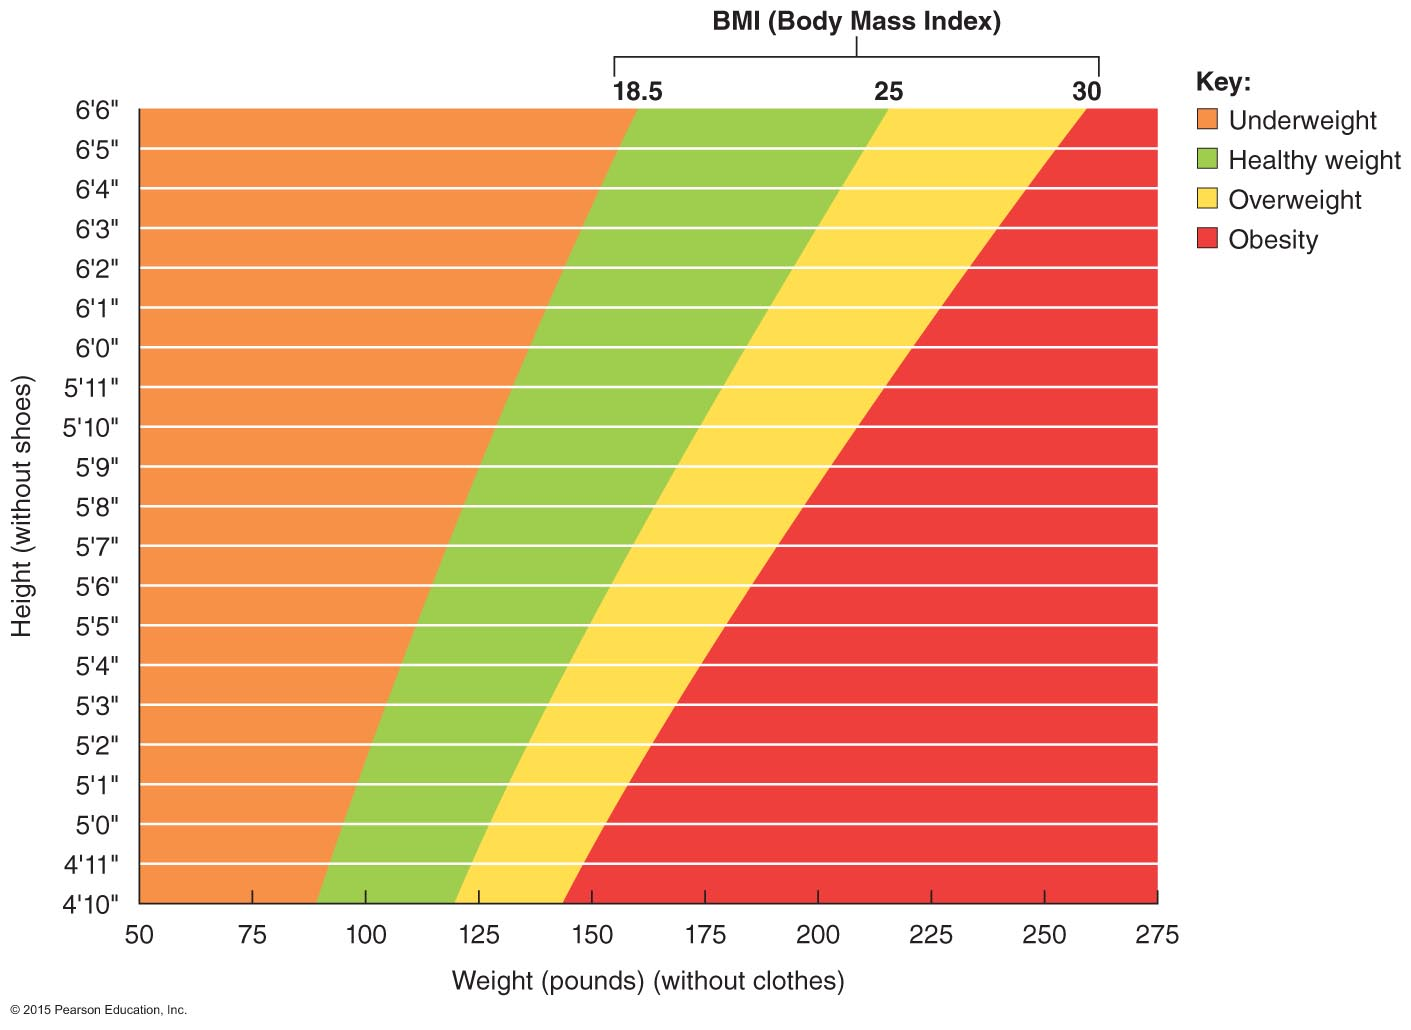
\includegraphics[width=\textwidth]{10_estimating_bmi}
	\caption{Estimating BMI}
	\label{fig:estimating-bmi}
\end{figure}

\begin{itemize}
	\item \definition{Underweight}{having too little body fat to maintain health}
	\item \definition{Overweight}{having a moderate amount of excess body fat}
	\item Normal weight: appropriate weight for height. Associated with the lowest disease risk
	\item \definition{Obesity}{having an excess of body fat that adversely affects health}
	\item \definition{Morbid obesity}{body weight exceeding 100\% of normal, creating a very high risk of serious health complications}
\end{itemize}

\section{Evaluating Body Weight}\label{sec:evaluating-body-weight2}
\begin{itemize}
	\item Body composition
	\begin{itemize}
		\item Measurement of body fat and lean body mass
		\item Can be measured by
		\begin{itemize}
			\item Underwater weighing
			\item Skinfold measurements
			\item Bioelectrical impedance analysis (BIA)
			\item Dual-energy x-ray absorptiometry (DXA)
			\item Bod Pod
		\end{itemize}
	\end{itemize}
\end{itemize}

\begin{figure}[H]
	\centering
	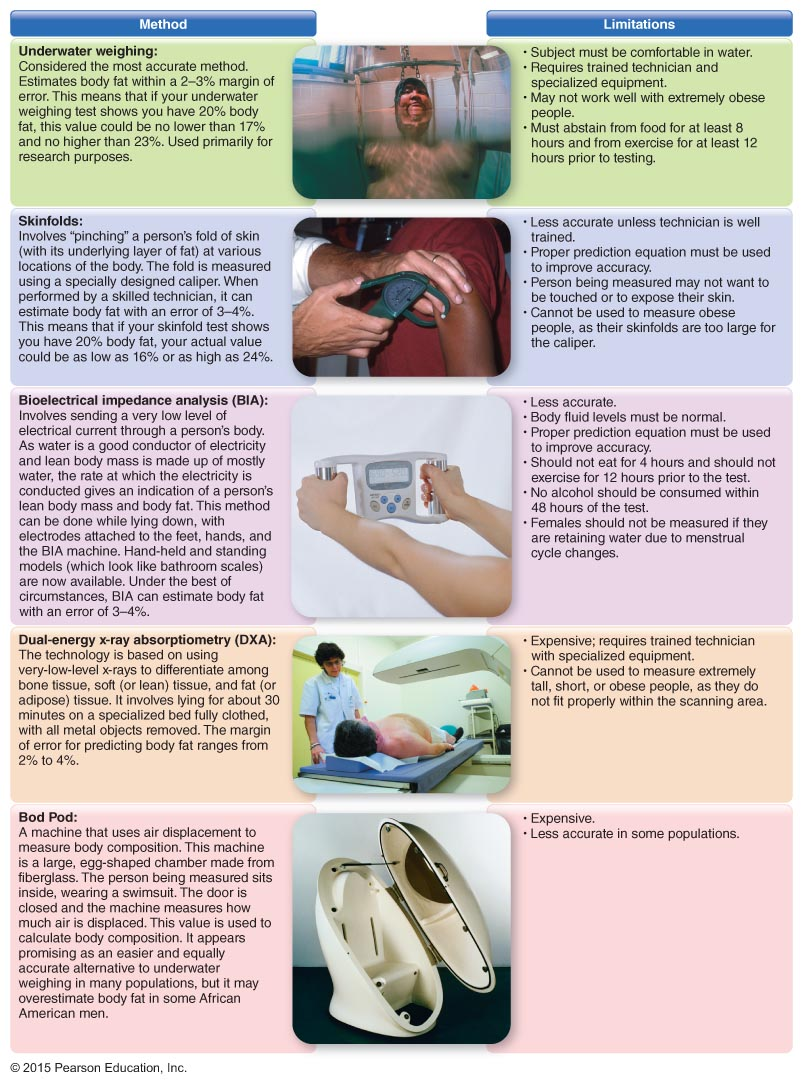
\includegraphics[width=\textwidth]{10_body_composition_assessment_methods}
	\caption{Body Composition Assessment Methods}
	\label{fig:body-composition-assessment-methods}
\end{figure}

\begin{itemize}
	\item Fat distribution pattern
	\begin{itemize}
		\item Measured by waist-to-hip ratio and waist circumference
		\begin{itemize}
			\item Disease risk is associated with a waist-to-hip ratio of higher than 0.90 in men, and 0.80 in women
		\end{itemize}
		\item \definition{Apple-shaped fat patterning}{upper body}
		\begin{itemize}
			\item Increased risk of chronic diseases (type 2 diabetes, heart disease, hypertension)
		\end{itemize}
		\item \definition{Pear-shaped fat patterning}{lower body}
		\begin{itemize}
			\item No significant increased risk of chronic diseases
		\end{itemize}
	\end{itemize}
\end{itemize}

\begin{figure}[H]
	\centering
	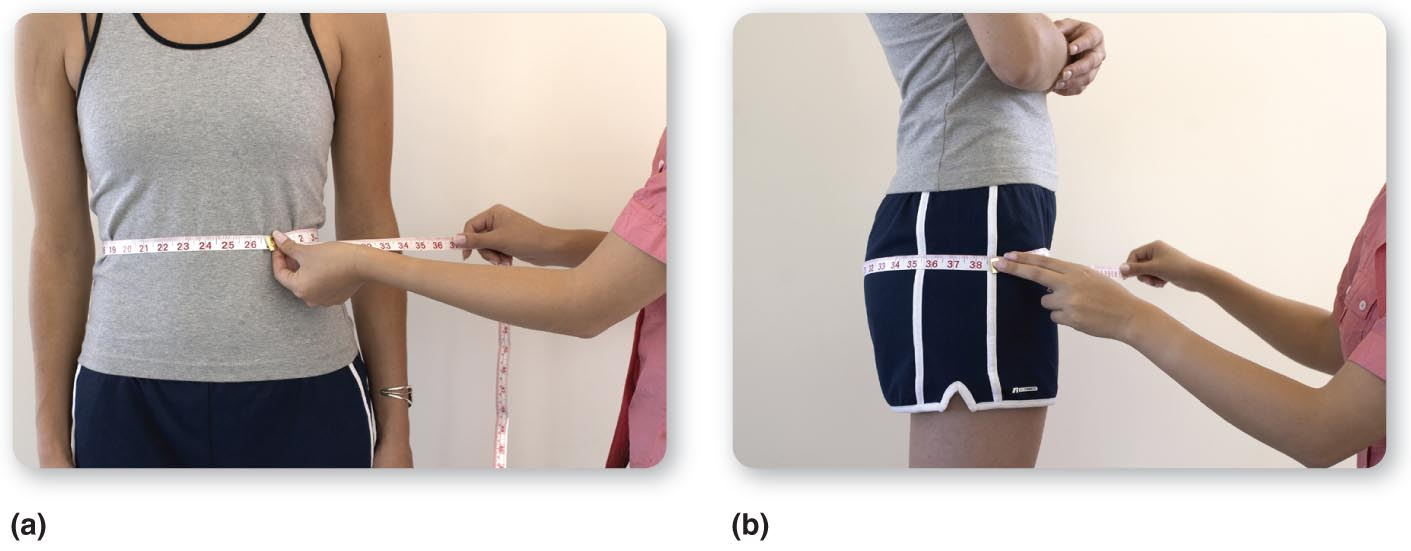
\includegraphics[height=0.75\paperheight]{10_determining_fat_patterning}
	\caption{Determining Fat Patterns}
	\label{fig:determining-fat-patterns}
\end{figure}

\section{Gaining or Losing Weight}\label{sec:gaining-or-losing-weight}
\begin{itemize}
	\item Whether a person gains or loses weight depends on
	\begin{itemize}
		\item Energy intake versus energy expenditure
		\item Genetic factors
		\item Composition of the diet
		\item Metabolic factors
		\item Physiologic factors
		\item Cultural and economic factors
		\item Social factors
	\end{itemize}
\end{itemize}

\section{Energy Balance}\label{sec:energy-balance}
\begin{itemize}
	\item Occurs when energy intake = energy expenditure
	\item Energy intake = kcal from food
	\item Energy expenditure
	\begin{itemize}
		\item Energy expended at rest (basal metabolic rate)
		\item Physical activity
		\item Thermic effect of food
	\end{itemize}
\end{itemize}

\begin{figure}[H]
	\centering
	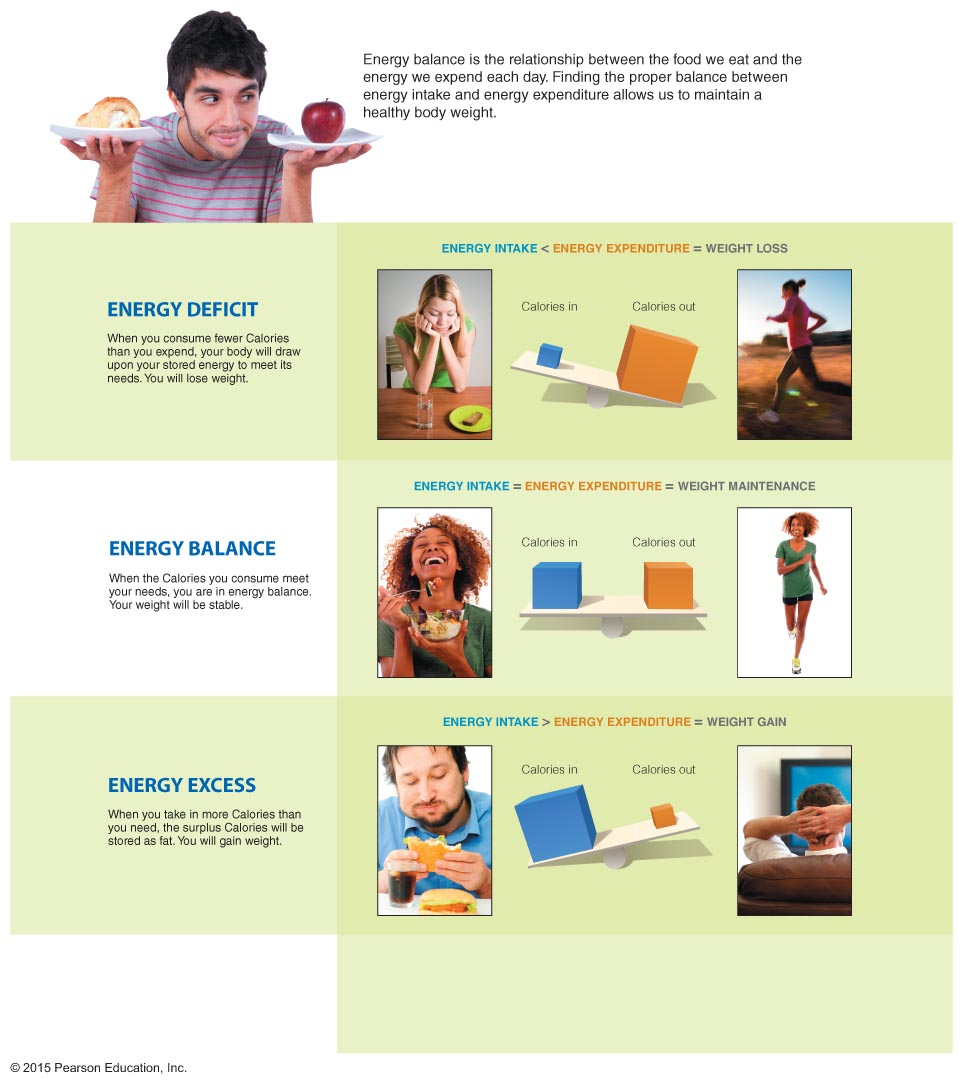
\includegraphics[width=\textwidth]{10_energy_balance}
	\caption{Energy Balance}
	\label{fig:energy-balance}
\end{figure}

\begin{itemize}
	\item Basal metabolic rate (BMR)
	\begin{itemize}
		\item Energy expended to maintain basal, or resting, functions of the body
		\item 60--75\% of total energy expenditure
		\item More lean tissue increases your BMR
		\item BMR decreases with age, 3--5\% per decade after age 30
	\end{itemize}
\end{itemize}

\begin{table}[H]
	\centering
	\caption{Factors Affecting Basal Metabolic Rate (BMR)}
	\label{tab:factors-affecting-bmr}
	\rowcolors{2}{rowmedgreen}{rowlightgreen}
	\begin{tabular}{p{0.5\textwidth}p{0.5\textwidth}}
		\rowcolor{rowdarkgreen}\textbf{Factors That Increase BMR} & \textbf{Factors That Decrease BMR}\\
		Higher lean body mass & Lower lean body mass\\
		Greater height (more surface area) & Lower height\\
		Younger age & Older age\\
		Elevated levels of thyroid hormone & Depressed levels of thyroid hormone\\
		Stress, fever, illness & Starvation, fasting or very-low-Calorie diets\\
		Male gender & Female gender (due to decreased lean tissue)\\
		Pregnancy and lactation & \\
		Certain drugs, such as stimulants, caffeine, and tobacco & \\
		\rowcolor{rowdarkgreen} & \\
	\end{tabular}
\end{table}

\begin{itemize}
	\item Thermic effect of food (TEF)
	\begin{itemize}
		\item Energy expended to digest, absorb, transport, metabolize, and store food
		\item 5--10\% of total expenditure
		\item Lowest for fat and highest for protein
	\end{itemize}
	\item Physical activity
	\begin{itemize}
		\item 15--35\% of daily energy expenditure
		\item Factors that influence energy expended
		\begin{itemize}
			\item The more muscle groups used, the greater the energy expenditure
			\item Intensity
			\item Duration
			\item Body size
		\end{itemize}
	\end{itemize}
\end{itemize}

\begin{table}[H]
	\centering
	\caption{Energy Costs of Physical Activities}
	\label{tab:energy-costs-of-physical-activities}
	\rowcolors{2}{rowmedgreen}{rowlightgreen}
	\begin{tabular}{p{0.7\textwidth}p{0.15\textwidth}p{0.15\textwidth}}
		\rowcolor{rowdarkgreen}\textbf{Activity} & \textbf{Intensity} & \textbf{Energy Cost (kcal/kg body weight/min)}\\
		Sitting, studying (including reading or writing) & Light & 0.022\\
		Cooking or food production (sitting or standing) & Light & 0.033\\
		Walking (e.g., to neighbor's house) & Light & 0.042\\
		Stretching--Hatha yoga & Moderate & 0.042\\
		Cleaning (dusting, straightening up, vacuuming, changing linen, carrying out trash) & Moderate & 0.058 \\
		Weight lifting (free weights, Nautilus or universal type) & Light or moderate & 0.050\\
		Bicycling, 10 mph & Leisure (work or pleasure) & 0.067\\
		Walking, 4 mph (brisk pace) & Moderate & 0.083\\
		Aerobics & Low impact & 0.083\\
		Weight lifting (free weights, Nautilus or universal type) & Vigorous & 0.100\\
		Bicycling, 12 to 13.9 mph & Moderate & 0.133\\
		Running, 5 mph (12 minutes per mile) & Moderate & 0.138\\
		Running, 6 mph (10 minutes per mile) & Moderate & 0.163\\
		Running, 8.6 mph (7 minutes per mile) & Vigorous & 0.205\\
		\rowcolor{rowdarkgreen} & & \\
	\end{tabular}
\end{table}

\section{Genetic Factors}\label{sec:genetic-factors}
\begin{itemize}
	\item Different ideas have been suggested to explain the impact of genetics on body fat
	\begin{itemize}
		\item FTO gene
		\item Thrifty gene theory
		\item Set-point theory
	\end{itemize}
\end{itemize}

\subsection{FTO gene}\label{subsec:fto-gene}
\begin{itemize}
	\item Fat mass and obesity-associated gene
	\item 44–65\% of people have at least one copy
	\item Stimulates excessive food intake
	\item Physical activity can attenuate the gene’s influence
\end{itemize}

\subsection{Thrifty gene theory}\label{subsec:thrifty-gene-theory}
\begin{itemize}
	\item Proposes that a gene (or genes) causes people to be energetically thrifty
	\item Proposes that people with this gene expend less energy than other people and therefore gain weight
	\item A ``thrifty gene'' has not been identified
\end{itemize}

\subsection{Set-point theory}\label{subsec:set-point-theory}
\begin{itemize}
	\item Proposes that each person’s weight stays within a small range (set point)
	\item The body compensates for changes in energy balance and keeps a person’s weight at his or her set point
	\item Can change with time, as diet and activity levels vary over a long period of time
\end{itemize}

\subsection{Protein leverage hypothesis}\label{subsec:protein-leverage-hypothesis}
\begin{itemize}
	\item Humans have evolved to have a fixed daily dietary protein target that must be reached to optimize physiologic functioning
	\item Diets high in carbohydrates and fats and low in protein may cause people to overeat
\end{itemize}

\subsection{Drifty gene hypothesis}\label{subsec:drifty-gene-hypothesis}
\begin{itemize}
	\item Suggests that in the new food environment some people become obese while others do not
	\item This effect may be due to random mutations and drift in genes that control upper body fatness
	\item These genes are originally thought to be neutral but over time and evolved to predispose us to obesity
\end{itemize}

\subsection{Metabolic Factors}\label{subsec:metabolic-factors}
\begin{itemize}
	\item Relatively low metabolic rate
	\item Low level of spontaneous physical activity
	\item Low sympathetic nervous system activity
	\item Low fat oxidation
	\item Low levels of thyroid hormones
	\item Certain prescription medications
\end{itemize}

\subsection{Physiologic Factors}\label{subsec:physiologic-factors}
\begin{itemize}
	\item Hunger and satiety
	\item Specific proteins and hormones
	\begin{itemize}
		\item Leptin
		\item Ghrelin
		\item Peptide YY, or PYY
		\item Brown adipose tissue
		\item Serotonin and cholecystokinin (CCK)
		\item Blood glucose levels
		\item Stomach expansion
		\item Nutrient absorption from the small intestine
		\item Beta-endorphins
		\item Neuropeptide Y
		\item Decreased blood glucose levels
	\end{itemize}
\end{itemize}

\subsection{Leptin}\label{subsec:leptin}
\begin{itemize}
	\item Leptin is a hormone produced by fat cells that causes reduced food intake, reduced weight, and decreased body fat in mice
	\item The role of leptin in human obesity is being studied
\end{itemize}

\subsection{Ghrelin}\label{subsec:ghrelin}
\begin{itemize}
	\item Protein synthesized in the stomach
	\item Stimulates appetite by acting on the hypothalamus
\end{itemize}

\subsection{Peptide YY, or PYY}\label{subsec:peptide-yy-or-pyy}
\begin{itemize}
	\item Produced in the GI tract
	\item Decreases appetite
	\item Obese people have lower levels when fasting
\end{itemize}

\subsection{Cultural and Economic Factors}\label{subsec:cultural-and-economic-factors}
\begin{itemize}
	\item Food choices
	\begin{itemize}
		\item The composition of a person’s diet should remain balanced
	\end{itemize}
	\item Levels of physical activity
	\begin{itemize}
		\item Minor changes can add up
	\end{itemize}
	\item Economic status
	\begin{itemize}
		\item Food choices and eating behaviors are affected
	\end{itemize}
	\item Cultural customs
	\item Changes in work and leisure activity levels
	\item Larger body size acceptance/cultural norms
	\item Lack of access to healthcare and health information
	\item Lack of access to affordable, healthful foods
	\item Lack of access to positive role models
	\item Personal safety issues
	\item Transportation issues
\end{itemize}

\section{Sociocultural Factors}\label{sec:sociocultural-factors}
\begin{itemize}
	\item Social factors influencing our diet and activity levels include
	\begin{itemize}
		\item Expectations of family and friends
		\item Holiday foods, fast foods, and serving sizes
		\item Television and other amusements that do not involve physical activity
		\item Work responsibilities that do not involve physical activity
		\item Media images and social pressures to achieve unrealistic weight goals
	\end{itemize}
\end{itemize}

\section{Achieve and Maintain Healthful Weight}\label{sec:achieve-and-maintain-healthful-weight}
\begin{itemize}
	\item Healthful weight change requires
	\item Gradual and reasonable changes in energy intake
	\item Regular and appropriate physical exercise
	\item Application of behavior modification techniques
\end{itemize}

\section{Diets focusing on Macronutrient Composition}\label{sec:diets-focusing-on-macronutrient-composition}
\begin{itemize}
	\item Diets high in carbohydrates and moderate fat and protein
	\begin{itemize}
		\item DASH diet, USDA Food Guide, Weight Watchers, and Jenny Craig
	\end{itemize}
	\item Diets low in carbohydrate and high in fat and protein
	\begin{itemize}
		\item Atkins, Sugar Busters!, and the Paleo diet
	\end{itemize}
\end{itemize}

\section{Weight-Loss Strategies}\label{sec:weight-loss-strategies}
\begin{itemize}
	\item Guidelines for successful weight loss
	\item \emph{Set realistic goals}
	\begin{itemize}
		\item Specific
		\item Reasonable
		\item Measurable
		\begin{itemize}
			\item Monitor progress regularly
		\end{itemize}
	\end{itemize}
	\item \emph{Eat smaller portions of lower-fat foods}
	\begin{itemize}
		\item Reduce consumption of high-fat and high-energy foods
		\item Consume foods high in nutrient density
	\end{itemize}
	\item \emph{Participate in regular physical activity}
	\begin{itemize}
		\item Critical for long-term maintenance of weight loss
	\end{itemize}
	\item \emph{Incorporate appropriate behavior modifications}
	\begin{itemize}
		\item Mindful eating: refers to a nonjudgmental awareness of emotional and physical sensations one experiences while eating
	\end{itemize}
\end{itemize}

\section{Behavior Modification}\label{sec:behavior-modification}
\begin{itemize}
	\item Mindful eating tips
	\begin{itemize}
		\item Focus only on eating
		\item Savor each bite
		\item Recruit all of your senses
		\item Pause and rest between bites
		\item Try 10 minutes of silence
	\end{itemize}
\end{itemize}

\begin{figure}[H]
	\centering
	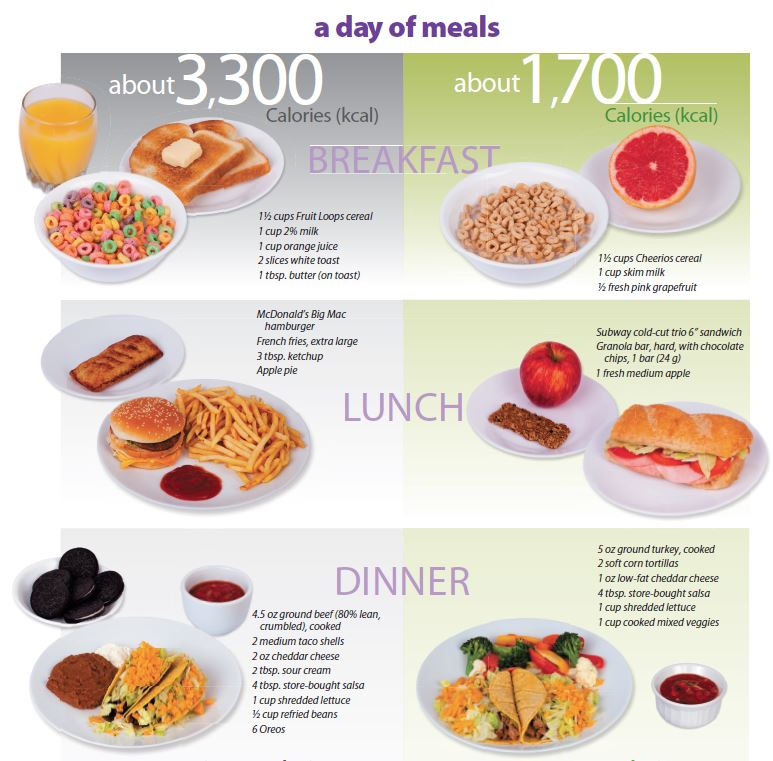
\includegraphics[width=\textwidth]{10_meals_energy_density}
	\caption{The Energy Density of Meals}
	\label{fig:meals-energy-density}
\end{figure}

\section{Underweight}\label{sec:underweight}
\begin{itemize}
	\item BMI below 18.5 kg/$\mbox{m}^{2}$
	\item Increases the risk of infections and illness
	\item Can be just as unhealthy as overweight
	\item Effective weight gain should include
	\begin{itemize}
		\item Eating 500 to 1,000 extra kcal/day
		\item Eating frequently throughout the day
		\item Selecting healthful, energy-dense foods
		\item Avoiding tobacco products, which depress appetite and increase BMR
		\item Regular exercise with resistance training
	\end{itemize}
\end{itemize}

\section{Obesity}\label{sec:obesity}
\begin{itemize}
	\item BMI between 30 and 39.9 kg/$\mbox{m}^{2}$
	\item Morbid obesity
	\begin{itemize}
		\item Body weight exceeding 100\% of normal
		\item BMI greater than or equal to 40 kg/$\mbox{m}^{2}$
	\end{itemize}
	\item Chronic diseases and complications linked to obesity include
	\begin{itemize}
		\item Hypertension
		\item Dislipidemia
		\item Type 2 diabetes
		\item Heart disease
		\item Stroke
		\item Gallbladder disease
		\item Osteoarthritis
		\item Sleep apnea
	\end{itemize}
	\item Chronic diseases and complications linked to obesity include
	\begin{itemize}
		\item Certain cancers
		\item Menstrual irregularities and infertility
		\item Gestational diabetes, premature fetal deaths, neural tube defects, and complications during labor and delivery
		\item Depression
		\item Alzheimer’s disease, dementia, and cognitive decline
	\end{itemize}
\end{itemize}

\begin{figure}[H]
	\centering
	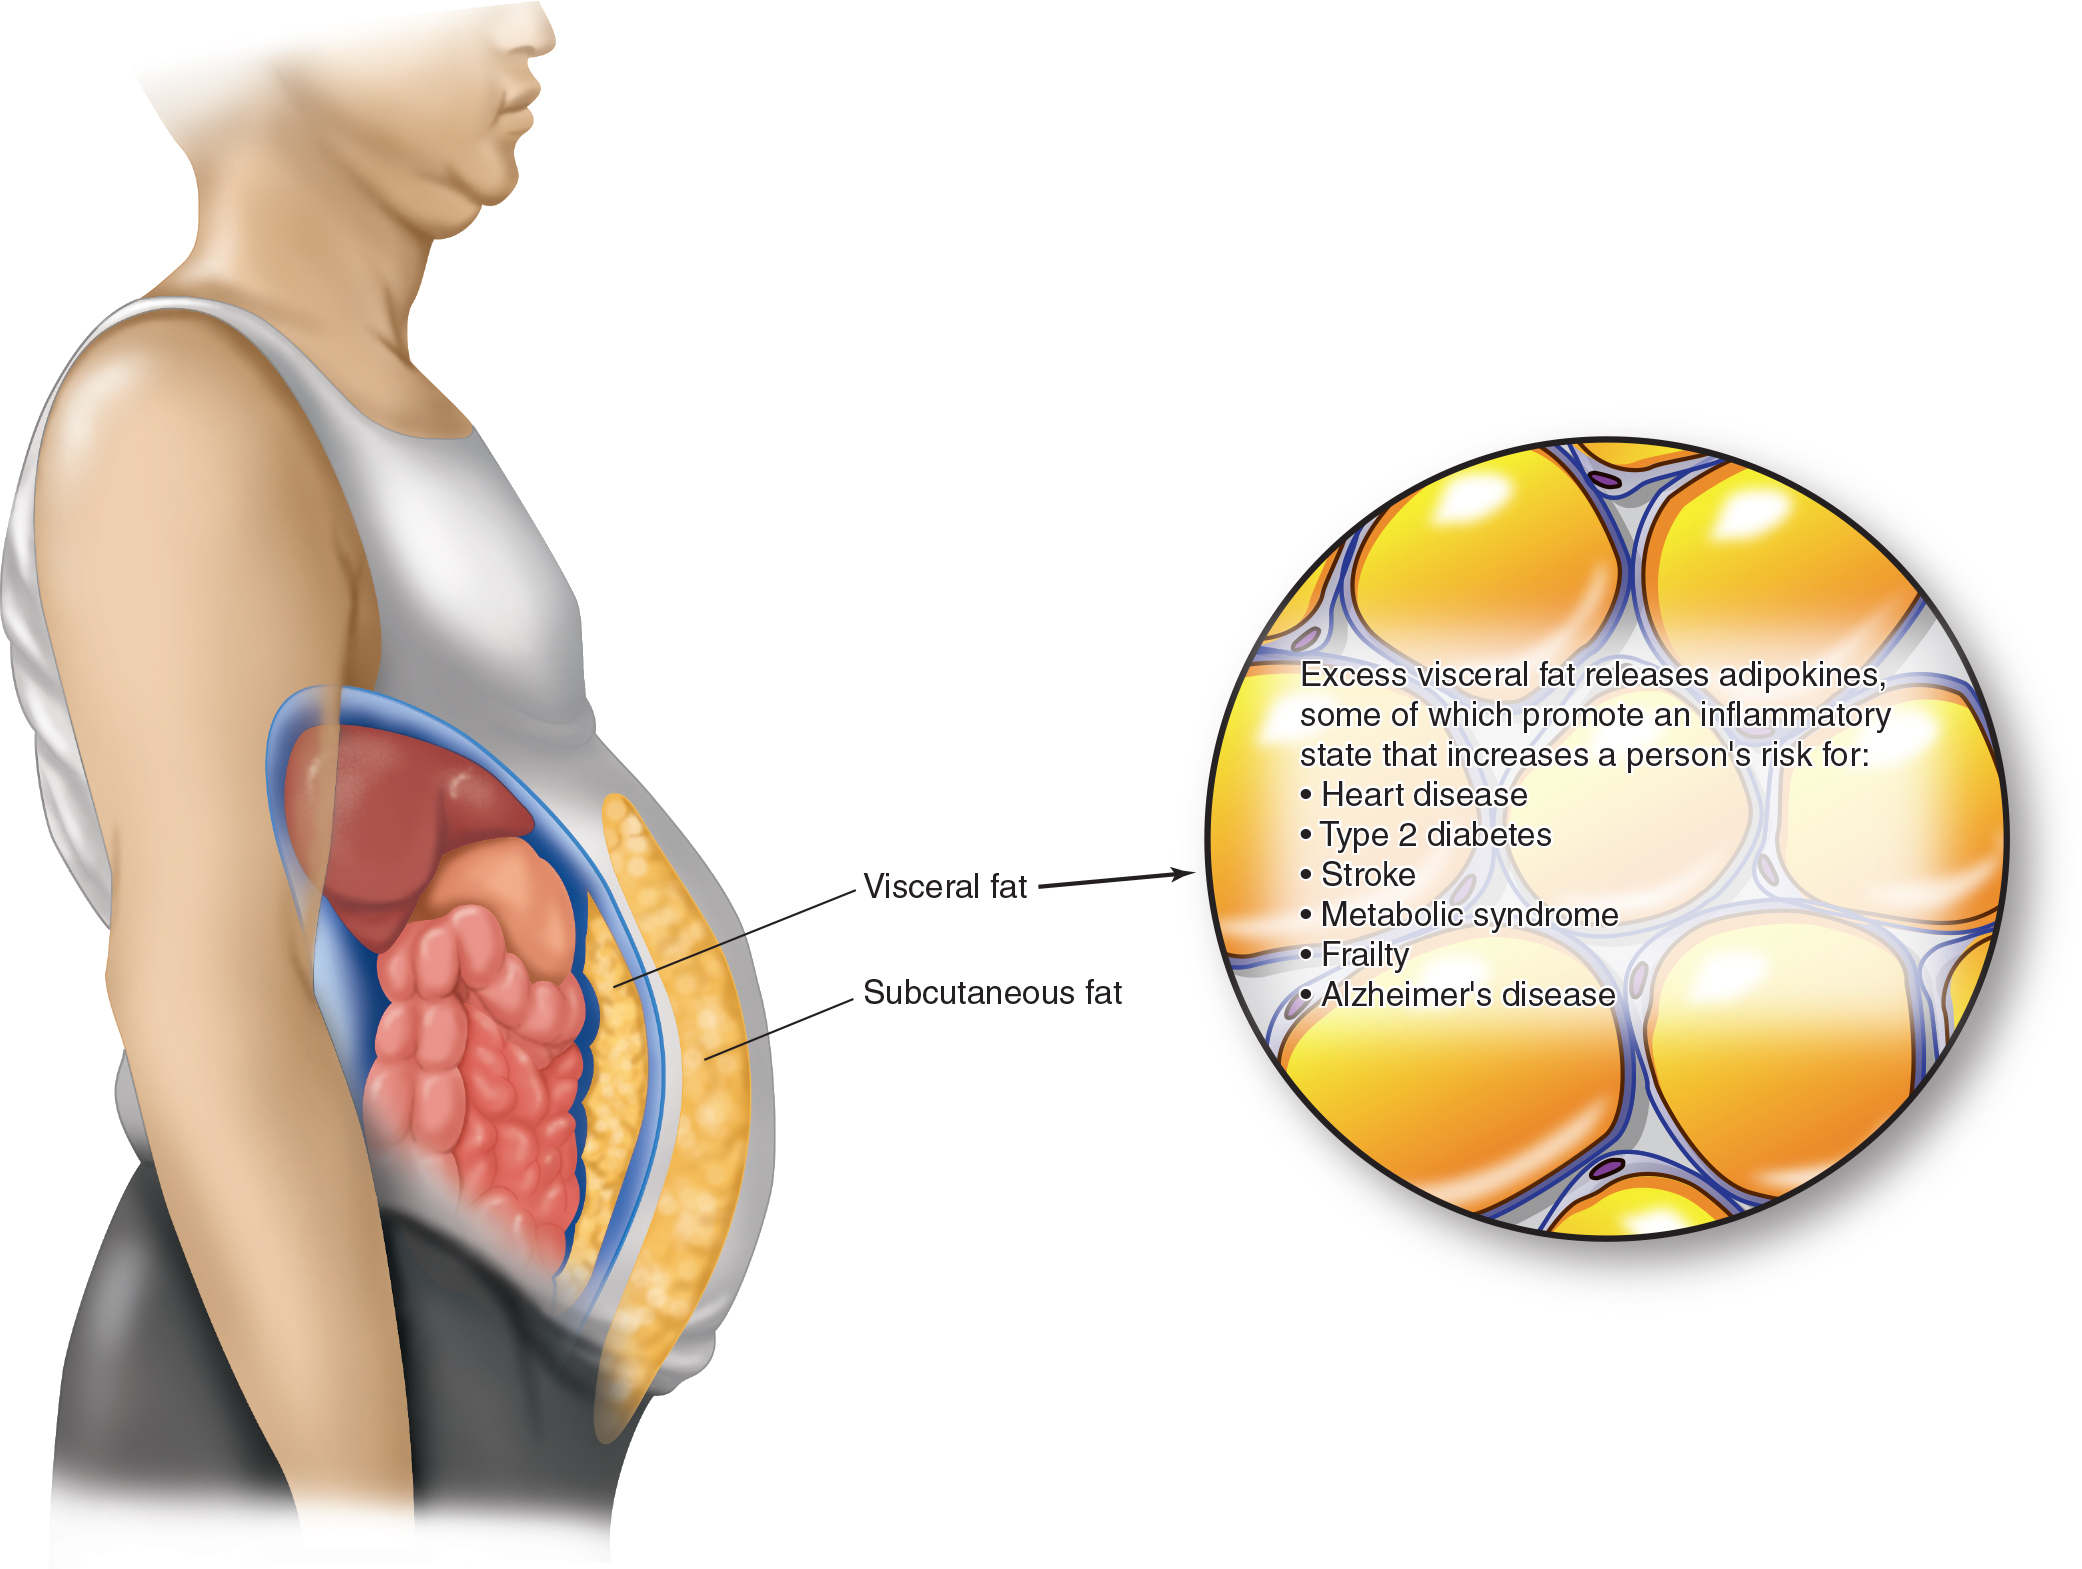
\includegraphics[width=\textwidth]{10_abdominal_obesity}
	\caption{Abdominal Obesity}
	\label{fig:abdominal-obesity}
\end{figure}

\subsection{Metabolic Syndrome}\label{subsec:metabolic-syndrome}
\begin{itemize}
	\item Abdominal obesity is one of the five risk factors of the metabolic syndrome
	\item People with metabolic syndrome are
	\begin{itemize}
		\item Twice as likely to develop heart disease
		\item Five times as likely to develop type 2 diabetes
	\end{itemize}
\end{itemize}

\begin{itemize}
	\item Factors that can influence the chance of developing obesity include
	\begin{itemize}
		\item Biology (genetics, metabolic, environment)
		\item Physical activity environment
		\item Individual physical activity
		\item Individual psychology
		\item Societal influences
		\item Food environment
		\item Food consumption
	\end{itemize}
\end{itemize}

\subsection{Obesity Responds to Diet and Exercise}\label{subsec:obesity-responds-to-diet-and-exercise}
\begin{itemize}
	\item Diet and exercise are the first line of defense against obesity
	\item Dietary and physical activity changes should be made gradually
	\item Physical activity for at least 30 minutes per day 5 days per week, but up to 60 minutes per day may be more beneficial for some people
\end{itemize}

\begin{itemize}
	\item Treatments for obesity may include
	\begin{itemize}
		\item Low-energy diet and regular exercise
		\item Counseling or psychotherapy
		\item Prescription medications
		\item Surgery
		\begin{itemize}
			\item Sleeve gastrectomy
			\item Gastric bypass
			\item Gastric banding
		\end{itemize}
	\end{itemize}
\end{itemize}

\begin{figure}[H]
	\centering
	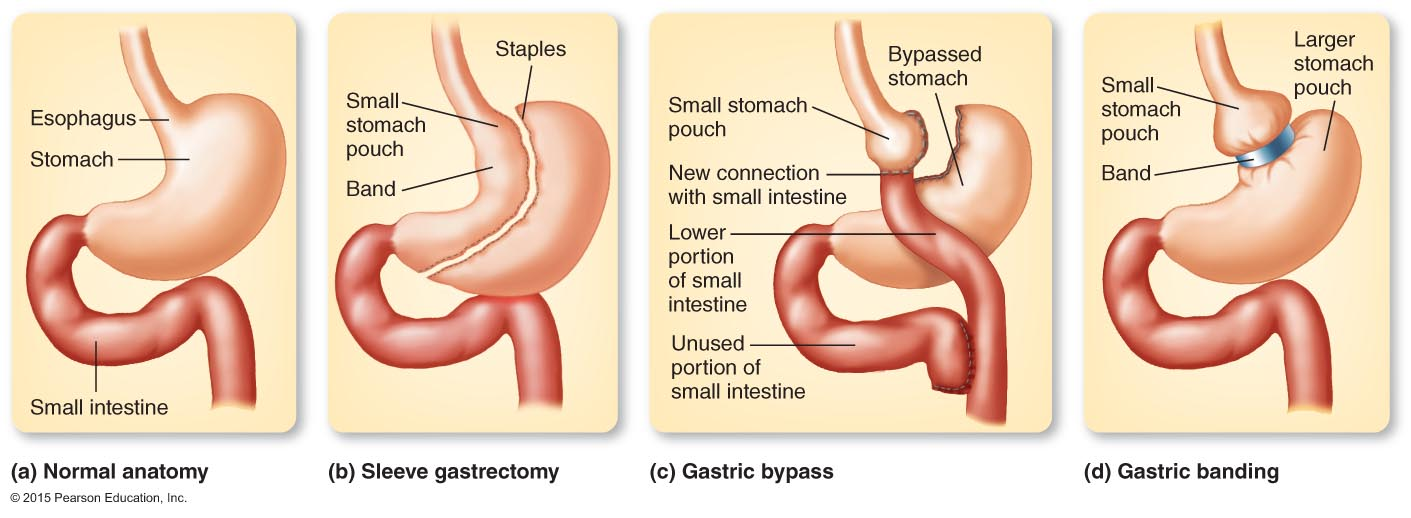
\includegraphics[width=\textwidth]{10_weight_loss_surgery}
	\caption{Weight-Loss Surgery}
	\label{fig:weight-loss-surgery}
\end{figure}


\end{document}
